\chapter{Un lecteur virtuel de codes-barres}

Après que l'application de test ait été achevée, je me retrouvai sans activité alors qu'il me restait la moitié de mon stage.
C'est ainsi que je me lançai dans un projet de détecteur virtuel de codes-barres.
Me basant sur le moteur de détection de GdPicture que je connaissais désormais, j'ai développé une application ergonomique et simple qui simule un lecteur de codes-barres sur des images ou des documents scannés.

\section{Objectifs}

Cette application devait tout d'abord reproduire le fonctionnement des lecteurs de codes-barres filaires existants.
Il devait être possible d'accéder rapidement à l'application depuis n'importe quelle autre, et que le lecteur soit une extension de la souris.
Enfin, plusieurs actions devaient être possibles une fois un code-barres détecté :
\begin{itemize}
\item Copier le résultat dans le presse-papier
\item Envoyer le résultat vers une autre fenêtre pour qu'elle le traite comme une entrée clavier
\end{itemize}

\section{Développement}

J'ai choisi de créer une application sans fenêtre, c'est à dire qui s'exécuterait d'une manière transparente pour l'utilisateur, et accessible depuis la zone de notifications\footnote{En anglais : \og system tray \fg{} ou plus simplement \og systray \fg{}}.
J'ai pour cela utilisé une bibliothèque WPF\footnote{Disponible ici : http://www.hardcodet.net/projects/wpf-notifyicon} prenant en charge cette fonctionnalité. Il m'est alors possible de créer une icône dans le systray, de créer un menu pour le clic-droit, de gérer les événements de clic et les info-bulles.

On peut voir dans la figure \ref{systrayMenu} le menu de l'application :
\begin{itemize}
\item Une case à cocher pour copier automatiquement le résultat d'une détection dans le presse-papiers
\item Una case à cocher pour l'envoyer dans une fenêtre.
\item Une liste pour choisir ladite fenêtre
\item Un bouton \og Plus d'options \fg{} qui ouvre une fenêtre permettant de choisir les types de codes-barres que l'on souhaite détecter.
\end{itemize}

\begin{figure}
\begin{center}
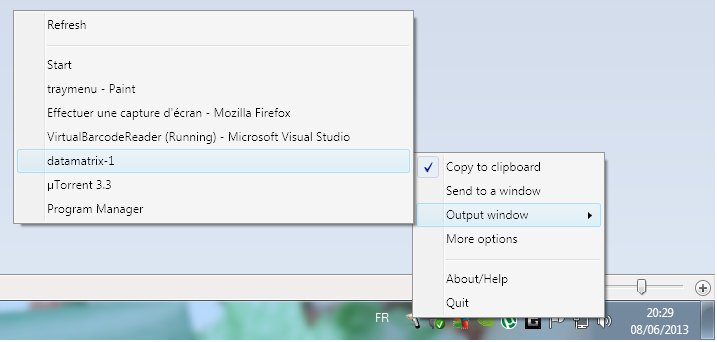
\includegraphics[scale=0.7]{images/traymenu.png}
\end{center}
\caption{Le lecteur de code-barres dans le systray}
\label{systrayMenu}
\end{figure}

\subsection{Envoyer des caractères à une autre application}

Une fonctionnalité intéressante du lecteur virtuel est de pouvoir définir une application vers laquelle seront redirigés les résultats des détections. Cela permet par exemple de remplir rapidement des formulaires en limitant le nombre de clics. Dans ce cas, je fais en sorte que le résultat soit envoyé à la fenêtre comme s'il avait été tapé au clavier.

[CODE]

\subsection{Gérer les intéractions pendant la détection}

Comme vous pouvez le constater dans la figure \ref{detectionRing}, le double-clic sur l'icône lance la détection matérialisée par un cercle. Pour détailler, il s'agit en fait d'une fenêtre dépouillée de son interface habituelle, dont le fond est transparent et dans laquelle une ellipse est dessinée.

\begin{figure}
\begin{center}
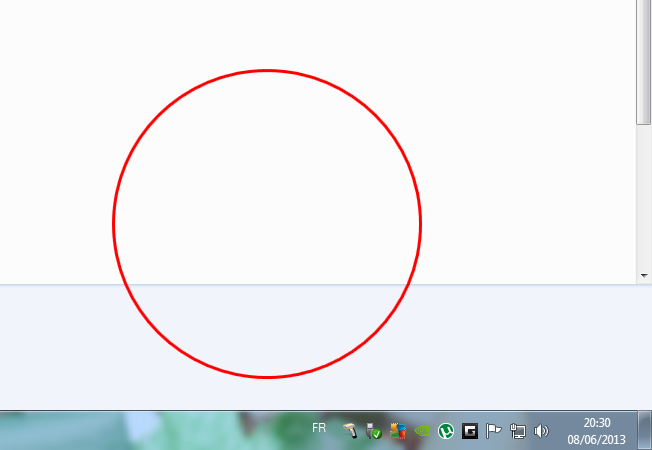
\includegraphics[scale=0.5]{images/detector.png}
\end{center}
\caption{Détection en cours}
\label{detectionRing}
\end{figure}

Grâce à des mécanismes avancés décris dans l'annexe \ref{detectionImage}, je peux récupérer certains événements utilisateurs comme le mouvement de la souris qui va provoquer le déplacement de la fenêtre de sorte que le curseur reste toujours au centre du cercle. Je vais aussi intercepter des événements plus complexes comme l'appui simultané des touches CTRL et MAJ et de la rotation de la molette de la souris. Cette action va permettre de faire varier la taille du cercle et donc la surface de détection. Je vais enfin intercepter tous les clics afin de m'assurer que le cercle reste en permanence au premier plan, sans quoi il serait vite perdu de vue derrière les autres fenêtres, sans possibilité de le ramener à l'avant-plan car la fenêtre ne possède pas d'icône dans la barre de tâche.

Le principe de la détection est de lancer à intervalle régulier une analyse de la zone survolée par le cercle de détection. Cette analyse consiste à capturer la zone de l'écran, à l'enregistrer dans une image en mémoire et à soumettre cette image à GdPicture en suivant le même principe que dans le premier projet que j'ai réalisé. Le choix des fonctions de détection à utiliser se fait cette fois-ci à l'aide des informations saisies par l'utilisateur dans la section \og Plus d'options \fg{}. En plus de la valeur du code-barres, je récupère son type afin de filtrer, toujours suivant les mêmes paramètres\footnote{En plus des types de détection habituels (DataMatrix, QRcode, etc.), il existe plusieurs familles de codes-barres 1D qui sont connues de GdPicture et qui peuvent être filtrées}.

Une fois qu'un code-barres est détecté, les actions automatiques se lancent si elles ont été activées. Il est toutefois possibles de les lancer manuellement :
\begin{itemize}
\item CTRL + MAJ + S pour envoyer le résultat à une fenêtre
\item CTRL + MAJ + D pour afficher une info-bulle contenant la valeur du code-barres
\item CTRL + MAJ + C pour copier le résultat dans le presse-papiers
\end{itemize}

\begin{figure}
\begin{center}
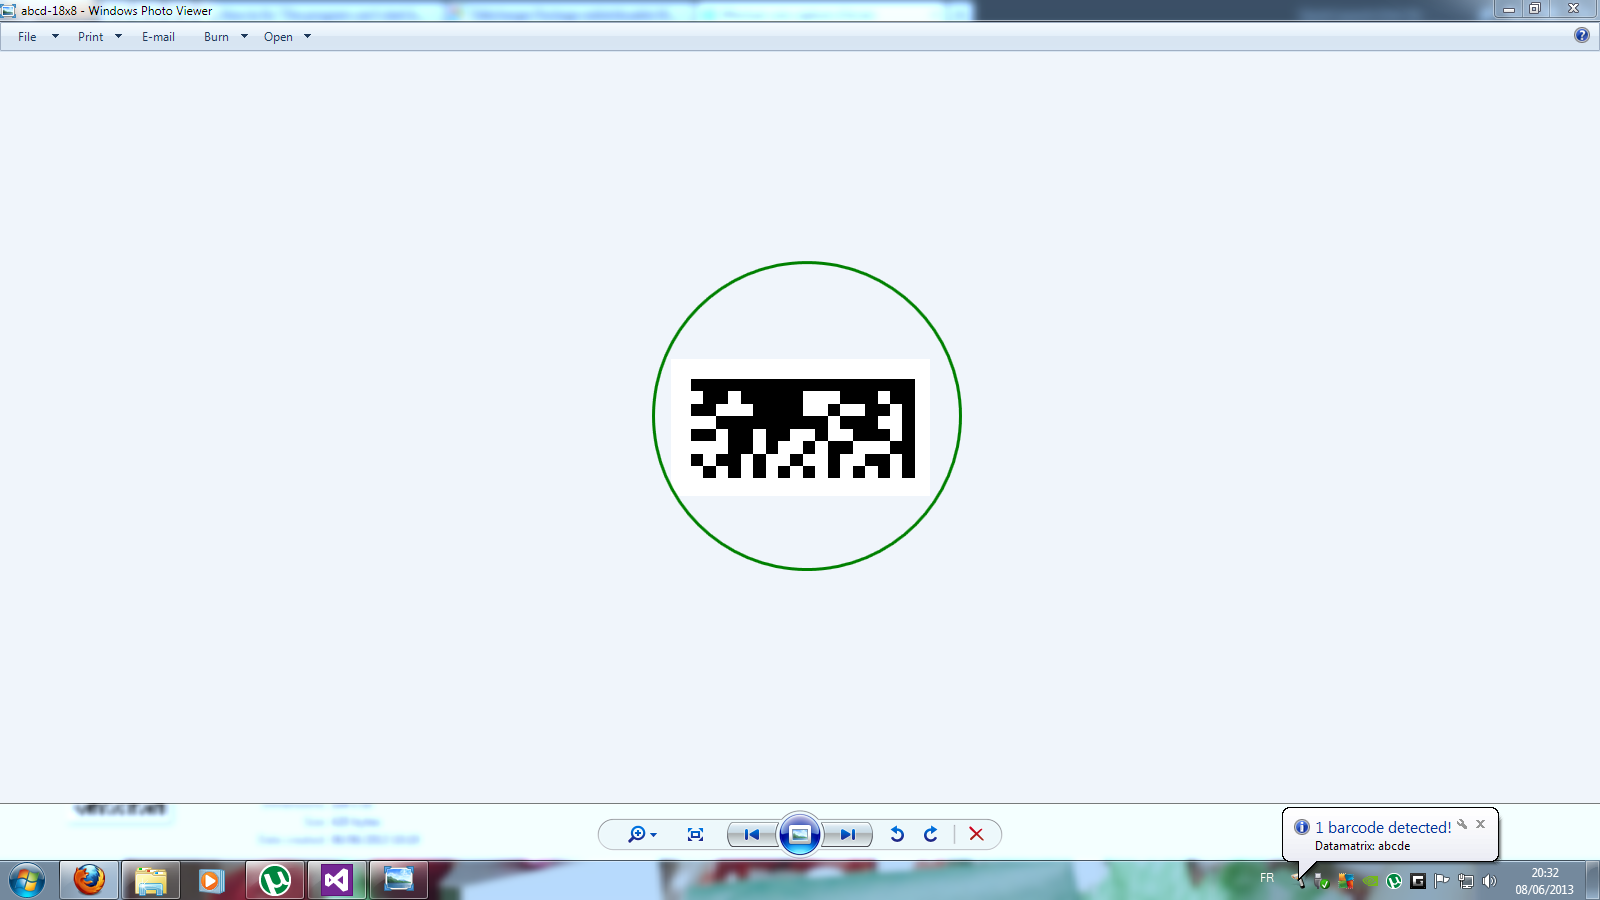
\includegraphics[scale=0.3]{images/detected.png}
\end{center}
\caption{1 code-barres détecté}
\label{detectedBarcode}
\end{figure}

\clearpage

\section{Bilan}

Ce second projet a été pour moi l'occasion d'approfondir mes connaissances dans les technologies que j'avais découvertes lors de mon premier projet. J'ai pu en effet mesurer mes progrès en relisant les premières lignes que j'avais écrites au début de mon stage, certaines me laissant dubitatif quant à leur qualité.

La réalisation de cete application m'a également permise de sortir du sujet initial de mon stage. J'ai pu me concentrer sur un sujet très différent, mais tout aussi intéressant. Malgré les longs moments passés à rechercher de la documentation sur certains mécanismes complexes, je garde le souvenir d'une application que je me suis amusé à créer.

Enfin, le lecteur de codes-barres virtuel est à destination du grand public, contrairement à l'application de tests. J'ai apprécié la volonté d'ORPALIS de supporter ce projet en le distribuant sur son site web sous le nom \og ORPALIS Virtual Barcode Reader \fg{} tout en laissant mon nom sur le produit.